%%%%%%%%%%%%%%%%%%%%%%%%%%%%%%%%%%%%%%%%%%%%%%%%%%%%%%%%%%%%%%%%%%%%%%%%%%%%%%%%%%%%%%%%%%%%%%%%%%%%%%%%%%%%%%%%%%%%%%%%%%%%%%%%%%%%%%%%%%%%%%%%%%%%%%%%%%%%%%%%%%%
% Written By Michael Brodskiy
% Class: Fundamentals of Linear Systems
% Professor: I. Salama
%%%%%%%%%%%%%%%%%%%%%%%%%%%%%%%%%%%%%%%%%%%%%%%%%%%%%%%%%%%%%%%%%%%%%%%%%%%%%%%%%%%%%%%%%%%%%%%%%%%%%%%%%%%%%%%%%%%%%%%%%%%%%%%%%%%%%%%%%%%%%%%%%%%%%%%%%%%%%%%%%%%

\include{Includes.tex}

\title{Homework 7}
\date{\today}
\author{Michael Brodskiy\\ \small Professor: I. Salama}

\begin{document}

\maketitle

\begin{enumerate}

  \item First and foremost, we see that the period is:

    $$T_o=6$$

    We know that the Fourier coefficient formula is given by:

    $$C_n=\frac{1}{T_o}\int_{-T_o/2}^{T_o/2}x(t)e^{-2\pi jnt/T_o}\,dt$$

    We substitute our known values to get:

    $$C_n=\frac{1}{6}\int_{-3}^{3} 2e^{-(\pi jnt)/3}\,dt$$
    $$C_n=\frac{1}{3}\int_{-1}^{1} e^{-(\pi jnt)/3}\,dt$$
    $$C_n=\frac{1}{3}\left(-\frac{3}{\pi jn} e^{-(\pi jnt)/3}\right)\Big|_{-1}^1$$

    We solve this to get:

    $$C_n=-\frac{1}{\pi jn} \left[e^{-(pi jn)/3} - e^{(\pi jn)/3}\right]$$
    $$\boxed{C_n=\frac{2}{n\pi}\sin\left( \frac{n\pi}{3} \right)}$$

    We then substitute to find the values given:

    $$\boxed{\left\{\begin{array}{ll} C_1&= .5513\\ C_2&= .2757\\ C_3&= 0\\ C_{-1}&= .5513\\ C_{-2}&= .2757\\C_{-3}&=0\end{array}}$$

      We then calculate $C_0$ separately:

      $$C_0=\frac{1}{6}\int_{-1}^{1}2\,dt$$
      $$C_0=\frac{1}{6}(2(1)-2(-1))$$
      $$\boxed{C_0=\frac{2}{3}}$$

  \item

    \begin{enumerate}

      \item We may use the transform table to write:

        $$Y(\omega)=\frac{j\omega}{(j\omega)^2+\omega_o^2}$$

        For a transform of $\cos(t)$. Combining this with the shifting property, we may write:

        $$\boxed{X(\omega)=\frac{j\omega + 3}{(j\omega+3)^2+25}}$$

      \item We may write the sinusoid as:

        $$Y(\omega)=\frac{\omega_o}{(j\omega)^2+\omega_o^2}$$

        We then apply the shifting property to get:

        $$X^1(\omega)=\frac{2}{(j\omega+1)^2+4}$$

        Finally, applying the $t$ term, we get:

        $$X(\omega)=j\frac{d}{d\omega}\left[ \frac{2}{(j\omega+1)^2+4} \right]$$
        $$X(\omega)=j\left[ \frac{2(-2j)}{[(j\omega+1)^2+4]^2} \right]$$
        $$\boxed{X(\omega)=\frac{4}{[(j\omega+1)^2+4]^2}}$$

    \end{enumerate}

  \item

    \begin{enumerate}

      \item We first list the relevant properties:

        $$x(t-t_o)\to e^{-j\omega t_o}X(j\omega)$$
        $$x(-t)\to X(-j\omega)$$

        Deconstructing the expression, we may write:

        $$X_1(\omega)=e^{-j\omega(4)}X(-j\omega)+e^{-j\omega(-4)}X(-j\omega)$$
        $$X_1(\omega)=X(-j\omega)[e^{-4j\omega}+e^{4j\omega}]$$

        We then use the property that:

        $$e^{-j\omega}+e^{j\omega}=2\cos(\omega)$$

        To get:

        $$\boxed{X_1(\omega)=2\cos(4\omega)X(-j\omega)}$$

      \item We first list the relevant properties:

        $$x(at)\to \frac{1}{|a|}X\left( \frac{j\omega}{a} \right)$$
        $$x(t-t_o)\to e^{-j\omega t_o}X(j\omega)$$
        $$tx(t)\to j\frac{d}{d\omega}[X(j\omega)]$$

        The expression given to us is of the form:

        $$x(t)=tx(at-t_o)$$

        Which lets us determine $a=3$ and $T_o=2$. As such, we obtain:

        $$X_2(\omega)=j\frac{d}{d\omega}\left[ \frac{e^{-2j\omega}}{3}X\left(\frac{j\omega}{3}\right) \right]$$
        $$\boxed{X_2(\omega)=\frac{j}{3}\frac{d}{d\omega}\left[ e^{-2j\omega}X\left(\frac{j\omega}{3}\right) \right]}$$

      \item First, we list the relevant properties:

        $$x(t-t_o)\to e^{-j\omega t_o}X(j\omega)$$
        $$x(-t)\to X(-j\omega)$$
        $$\frac{d}{dt}[x(t)]=j\omega X(j\omega)$$

        From this, we determine that $X(j\omega)\to X(-j\omega)$, and that the signal is time-shifted by $e^{-j\omega}$. Furthermore, it is multiplied by $(j\omega)^2$. Putting this all together, we see:

        $$\boxed{X_3(j\omega)=-\omega^2e^{-j\omega}X(-j\omega)}$$

    \end{enumerate}

  \item

    \begin{enumerate}

      \item First, we see that the transform is:

        $$\boxed{X_1(j\omega)=\frac{1}{2+j\omega}}$$

      \item Then, we see that:

        $$\boxed{X_1(-j\omega)=\frac{1}{2-j\omega}}$$

      \item Synthesizing parts (a) and (b), we may say that:

        $$\mathcal{F}\left\{ e^{-2|t|} \right\}=X_1(j\omega)+X_1(-j\omega)$$

        This gives us:

        $$\boxed{\mathcal{F}\left\{ e^{-2|t|} \right\}=\frac{1}{2+j\omega}+\frac{1}{2-j\omega}}$$

        Note that this may be written as:

        $$\boxed{\mathcal{F}\left\{ e^{-2|t|} \right\}=\frac{4}{4+\omega^2}}$$

      \item Using the table, we find that:

        $$\boxed{\mathcal{F}\left\{ \sin(5t) \right\}=\frac{\pi}{j}\left[ \delta(\omega-5)-\delta(\omega+5) \right]}$$

      \item Combining parts (a) through (d), we may see that, with $x(t)$:

        $$x(t)=e^{-2|t|}\sin(5t)$$

        The transform becomes:

        $$\mathcal{F}\left\{ e^{-2t}\sin(5t)u(t)-e^{2t}\sin(5t)u(-t) \right\}$$

        We see the first term transforms as:

        $$\left[ \frac{\pi}{j}\left( \frac{1}{2+j(\omega-5)}-\frac{1}{2+j(\omega+5)} \right) \right]-\mathcal{F}\left\{ e^{2t}\sin(5t)u(-t) \right\}$$

        And then we may find the full transform as:

        $$\boxed{X(j\omega)=\frac{\pi}{j}\left[ \left( \frac{1}{2+j(\omega-5)}-\frac{1}{2+j(\omega+5)} \right) -\left( \frac{1}{2-j(\omega-5)}-\frac{1}{2-j(\omega+5)} \right)\right]}$$

    \end{enumerate}

  \item

    \begin{enumerate}

      \item We may find the derivative to be:

        $$\boxed{\dot{x}(t)=-\delta(t)+u(t-1)-u(t-3)-\delta(t-4)}$$

      \item Taking the differential with respect to time of $p_T(t)$ as $\dot{p}_T(t)$, we may write:

        $$\boxed{\dot{x}(t)=p_1(t-2)-\dot{p}_2(t-1)}$$

      \item Rewriting in terms of $\delta$ and the rectangle function, we get:

        $$\dot{x}(t)=\text{rect}\left( \frac{t-2}{2} \right)-\delta(t)-\delta(t-4)$$

        From the table, we get:

        $$\boxed{\dot{X}(j\omega)=\frac{2\sin(\omega)}{\omega}e^{-2j\omega}-1-e^{-4j\omega}}$$

      \item Per the properties of Fourier transforms, we know that:

        $$\frac{d}{dt}[x(t)]=j\omega X(j\omega)$$

        This gives us:

        $$\boxed{X(j\omega)=\frac{2\sin(\omega)}{j\omega^2}e^{-2j\omega}-\frac{1}{j\omega}-\frac{e^{-4j\omega}}{j\omega}}$$

    \end{enumerate}

  \item

    \begin{enumerate}

      \item Per the frequency shifting property, we know:

        $$e^{j\omega_ot}x(t)\longleftrightarrow X(j(\omega-\omega_o))$$

        From our table of transforms, we know:

        $$x(t)\longleftrightarrow X(j\omega)\quad\text{ and }\quad e^{j\omega_ot}\longleftrightarrow 2\pi\delta(\omega-\omega_o)$$

        Combining these, we find:

        $$e^{j\omega_ot}x(t)=\frac{1}{2\pi}\left[ X(j\omega)\cdot2\pi\delta(\omega-\omega_o) \right]$$

        This is equivalent to:

        $$e^{j\omega_ot}x(t)= X(j\omega)\cdot\delta(\omega-\omega_o) $$

        Per the sifting property, we may conclude the frequency shifting property by getting:

      $$\boxed{e^{j\omega_ot}x(t)= X(j(\omega-\omega_o))}$$

    \item Given that $y(t)=2\cos(\omega_ot)x(t)$, we may write:

      $$y(t)=[e^{j\omega_ot}+e^{-j\omega_o t}]x(t)$$

      Per the frequency property determined in (a), we may write:

      $$\boxed{Y(j\omega)=X(j(\omega-\omega_o))+X(j(\omega+\omega_o))}$$

    \item From the result in part (b), we may determine:

      $$Y_1(j\omega)=.5[X(j(\omega-3))+X(j(\omega+3))]$$
      $$Y_2(j\omega)=.5[X(j(\omega-.5))+X(j(\omega+.5))]$$

      This gives us the following plots:

      \begin{figure}[H]
        \centering
        \tikzset{every picture/.style={line width=0.75pt}} %set default line width to 0.75pt        

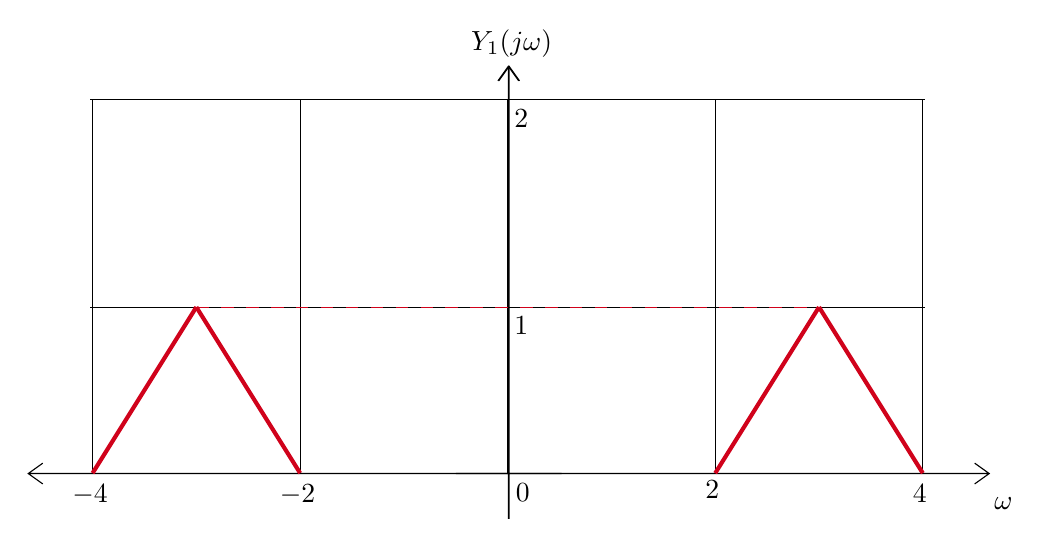
\begin{tikzpicture}[x=0.75pt,y=0.75pt,yscale=-1,xscale=1]
%uncomment if require: \path (0,590); %set diagram left start at 0, and has height of 590

%Shape: Axis 2D [id:dp039547207268332385] 
\draw  (277,252.2) -- (534,252.2)(302.7,56) -- (302.7,274) (527,247.2) -- (534,252.2) -- (527,257.2) (297.7,63) -- (302.7,56) -- (307.7,63)  ;
%Shape: Grid [id:dp9841770007230126] 
\draw  [draw opacity=0] (302,72) -- (503,72) -- (503,252) -- (302,252) -- cycle ; \draw   (302,72) -- (302,252)(402,72) -- (402,252)(502,72) -- (502,252) ; \draw   (302,72) -- (503,72)(302,172) -- (503,172) ; \draw    ;
%Shape: Axis 2D [id:dp9362667242858227] 
\draw  (328,252.2) -- (71,252.2)(302.3,56) -- (302.3,274) (78,247.2) -- (71,252.2) -- (78,257.2) (307.3,63) -- (302.3,56) -- (297.3,63)  ;
%Shape: Grid [id:dp6769124018924975] 
\draw  [draw opacity=0] (302,72) -- (101,72) -- (101,252) -- (302,252) -- cycle ; \draw   (302,72) -- (302,252)(202,72) -- (202,252)(102,72) -- (102,252) ; \draw   (302,72) -- (101,72)(302,172) -- (101,172) ; \draw    ;
%Straight Lines [id:da044228377793803286] 
\draw [color={rgb, 255:red, 208; green, 2; blue, 27 }  ,draw opacity=1 ][line width=1.5]    (102,252) -- (152,172) ;
%Straight Lines [id:da18764857256530187] 
\draw [color={rgb, 255:red, 208; green, 2; blue, 27 }  ,draw opacity=1 ][line width=1.5]    (402,252) -- (452,172) ;
%Straight Lines [id:da32221137112107656] 
\draw [color={rgb, 255:red, 208; green, 2; blue, 27 }  ,draw opacity=1 ][line width=1.5]    (202,252) -- (152,172) ;
%Straight Lines [id:da7356659104367959] 
\draw [color={rgb, 255:red, 208; green, 2; blue, 27 }  ,draw opacity=1 ][line width=1.5]    (502,252) -- (452,172) ;
%Straight Lines [id:da02923480394023481] 
\draw [color={rgb, 255:red, 208; green, 2; blue, 27 }  ,draw opacity=1 ] [dash pattern={on 4.5pt off 4.5pt}]  (152,172) -- (452,172) ;

% Text Node
\draw (304,175.4) node [anchor=north west][inner sep=0.75pt]    {$1$};
% Text Node
\draw (304,75.4) node [anchor=north west][inner sep=0.75pt]    {$2$};
% Text Node
\draw (396,254.4) node [anchor=north west][inner sep=0.75pt]    {$2$};
% Text Node
\draw (496,256.4) node [anchor=north west][inner sep=0.75pt]    {$4$};
% Text Node
\draw (191,256.4) node [anchor=north west][inner sep=0.75pt]    {$-2$};
% Text Node
\draw (91,256.4) node [anchor=north west][inner sep=0.75pt]    {$-4$};
% Text Node
\draw (304.7,255.6) node [anchor=north west][inner sep=0.75pt]    {$0$};
% Text Node
\draw (303.9,52.98) node [anchor=south] [inner sep=0.75pt]    {$Y_{1}( j\omega )$};
% Text Node
\draw (540.9,270.98) node [anchor=south] [inner sep=0.75pt]    {$\omega $};


\end{tikzpicture}

        \caption{Plot for $Y_1(j\omega)$}
        \label{fig:1}
      \end{figure}

      \begin{figure}[H]
        \centering
        \include{Figures/HW7-6c2}
        \caption{Plot for $Y_2(j\omega)$}
        \label{fig:2}
      \end{figure}

  \end{enumerate}

  \item

    \begin{enumerate}

      \item From our result in Problem 7 part (b), we may write this as:

        $$Y(j\omega)=\frac{1}{2}\left[ X(j(\omega-2))+X(j(\omega+2)) \right]$$

        We may re-express the given transform of $Y$ as:

        $$Y(j\omega)=u(t+4)-u(t-4)$$

        Equating the two, we get:

        $$2u(t+4)-2u(t-4)=X(j(\omega-2))+X(j(\omega+2))$$

        Thus, we see that we may write this as:

        $$\boxed{X(j\omega)=\left\{\begin{array}{ll}2,&|\omega|<2\\0,&\text{otherwise}\end{array}}$$

        Alternatively, we may write this as:

        $$X(j\omega)=2u(t+2)-2u(t-2)$$

        This gives us:

        $$x(t)=\frac{1}{2\pi}\int_{-\infty}^{\infty}X(j\omega)e^{j\omega t}\,d\omega$$
        $$x(t)=\frac{1}{\pi}\int_{-2}^{2}e^{j\omega t}\,d\omega$$
        $$x(t)=\frac{1}{\pi}\left[\frac{e^{j\omega t}}{j t}\right]\Big|_{-2}^{2}$$
        $$x(t)=\frac{e^{2jt}-e^{-2jt}}{j\pi t}$$

        This can be simplified to get:

        $$\boxed{x(t)=\frac{2\sin(2t)}{\pi t}}$$

      \item $x(t)\cos(t)$ may be plotted as:

        \begin{figure}[H]
          \centering
          \includegraphics[width=.8\textwidth]{Figures/HW7-7b}
          \caption{Plot of $x(t)\cos(t)$}
          \label{fig:3}
        \end{figure}

    \end{enumerate}

  \item

    \begin{enumerate}

      \item We are given that the signal is real, finite, and has even symmetry. Per properties of Fourier transforms, this means that the transform is real and even as well (the imaginary part is zero, and phase is zero). If the transform is real and has even symmetry, then the magnitude of the transform will also have even symmetry. Thus, we may look at the figure and see that this is only true for $X_4(j\omega)$ and $X_5(j\omega)$.

      \item We are given that the signal is real, finite, and has odd symmetry. This means that the Fourier transform must be imaginary and odd. This means that the phase needs to be $\pm\pi/2$, and the magnitude of the transform must have even symmetry. Looking at our options, we see that this is true only for $X_3(j\omega)$ and $X_6(j\omega)$.

    \end{enumerate}

\end{enumerate}

\end{document}

